\section{Methodology Overview}

The general processing steps performed in this work can be grouped
into four processing stages, or workflows. A simplified overview of
these stages and the flow of data between them is shown in Figure
\ref{fig:simple-work}. In ascending order, each processing stage is
discussed in more detail in Sections \ref{met:seq-workflow},
\ref{met:predict-workflow}, \ref{met:valid-workflow}, and
\ref{section:region-met}.

\begin{figure}
  \centering
  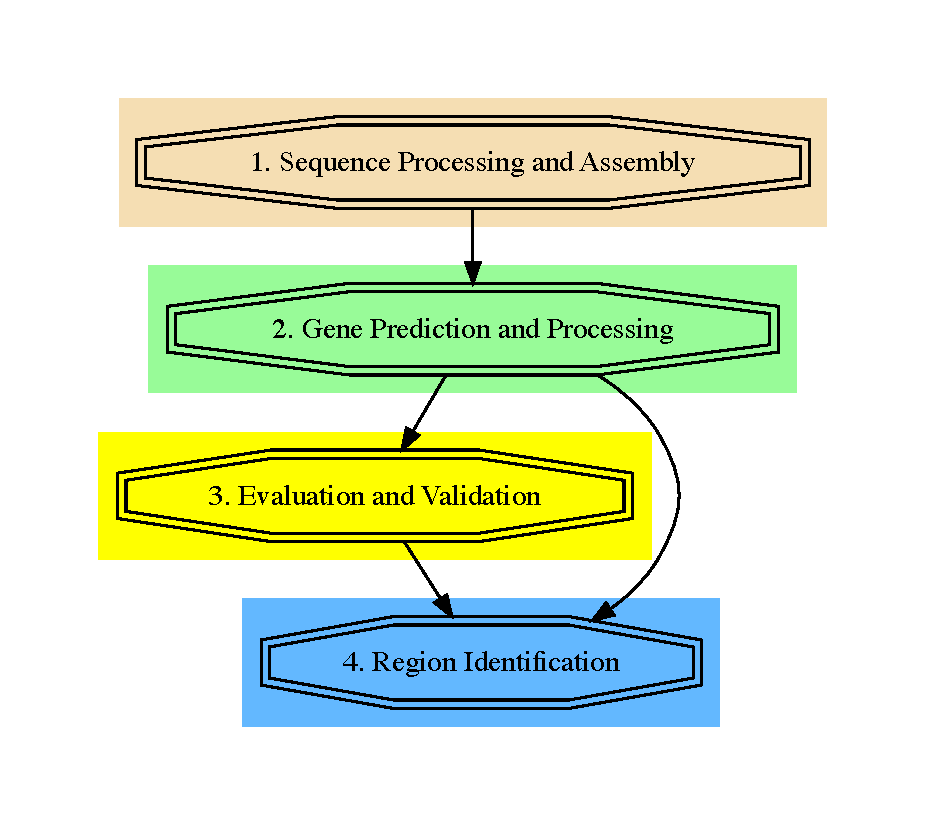
\includegraphics[width=0.8\textwidth]{figures/workflow-simple.pdf}
  \caption{A simplified workflow used in this work. Each processing
    stage is is represented by an octagon, and the flow of data are
    indicated by directed edges between them. In this figure and
    subsequent figures, the sequence processing stage is coloured
    brown, the gene prediction and processing stage is coloured green,
    the evaluation and validation stage is coloured yellow, and the
    region identification process is coloured blue.}
  \label{fig:simple-work}
\end{figure}

%\begin{figure}
%  \centering
%  \makebox[0pt]{
%    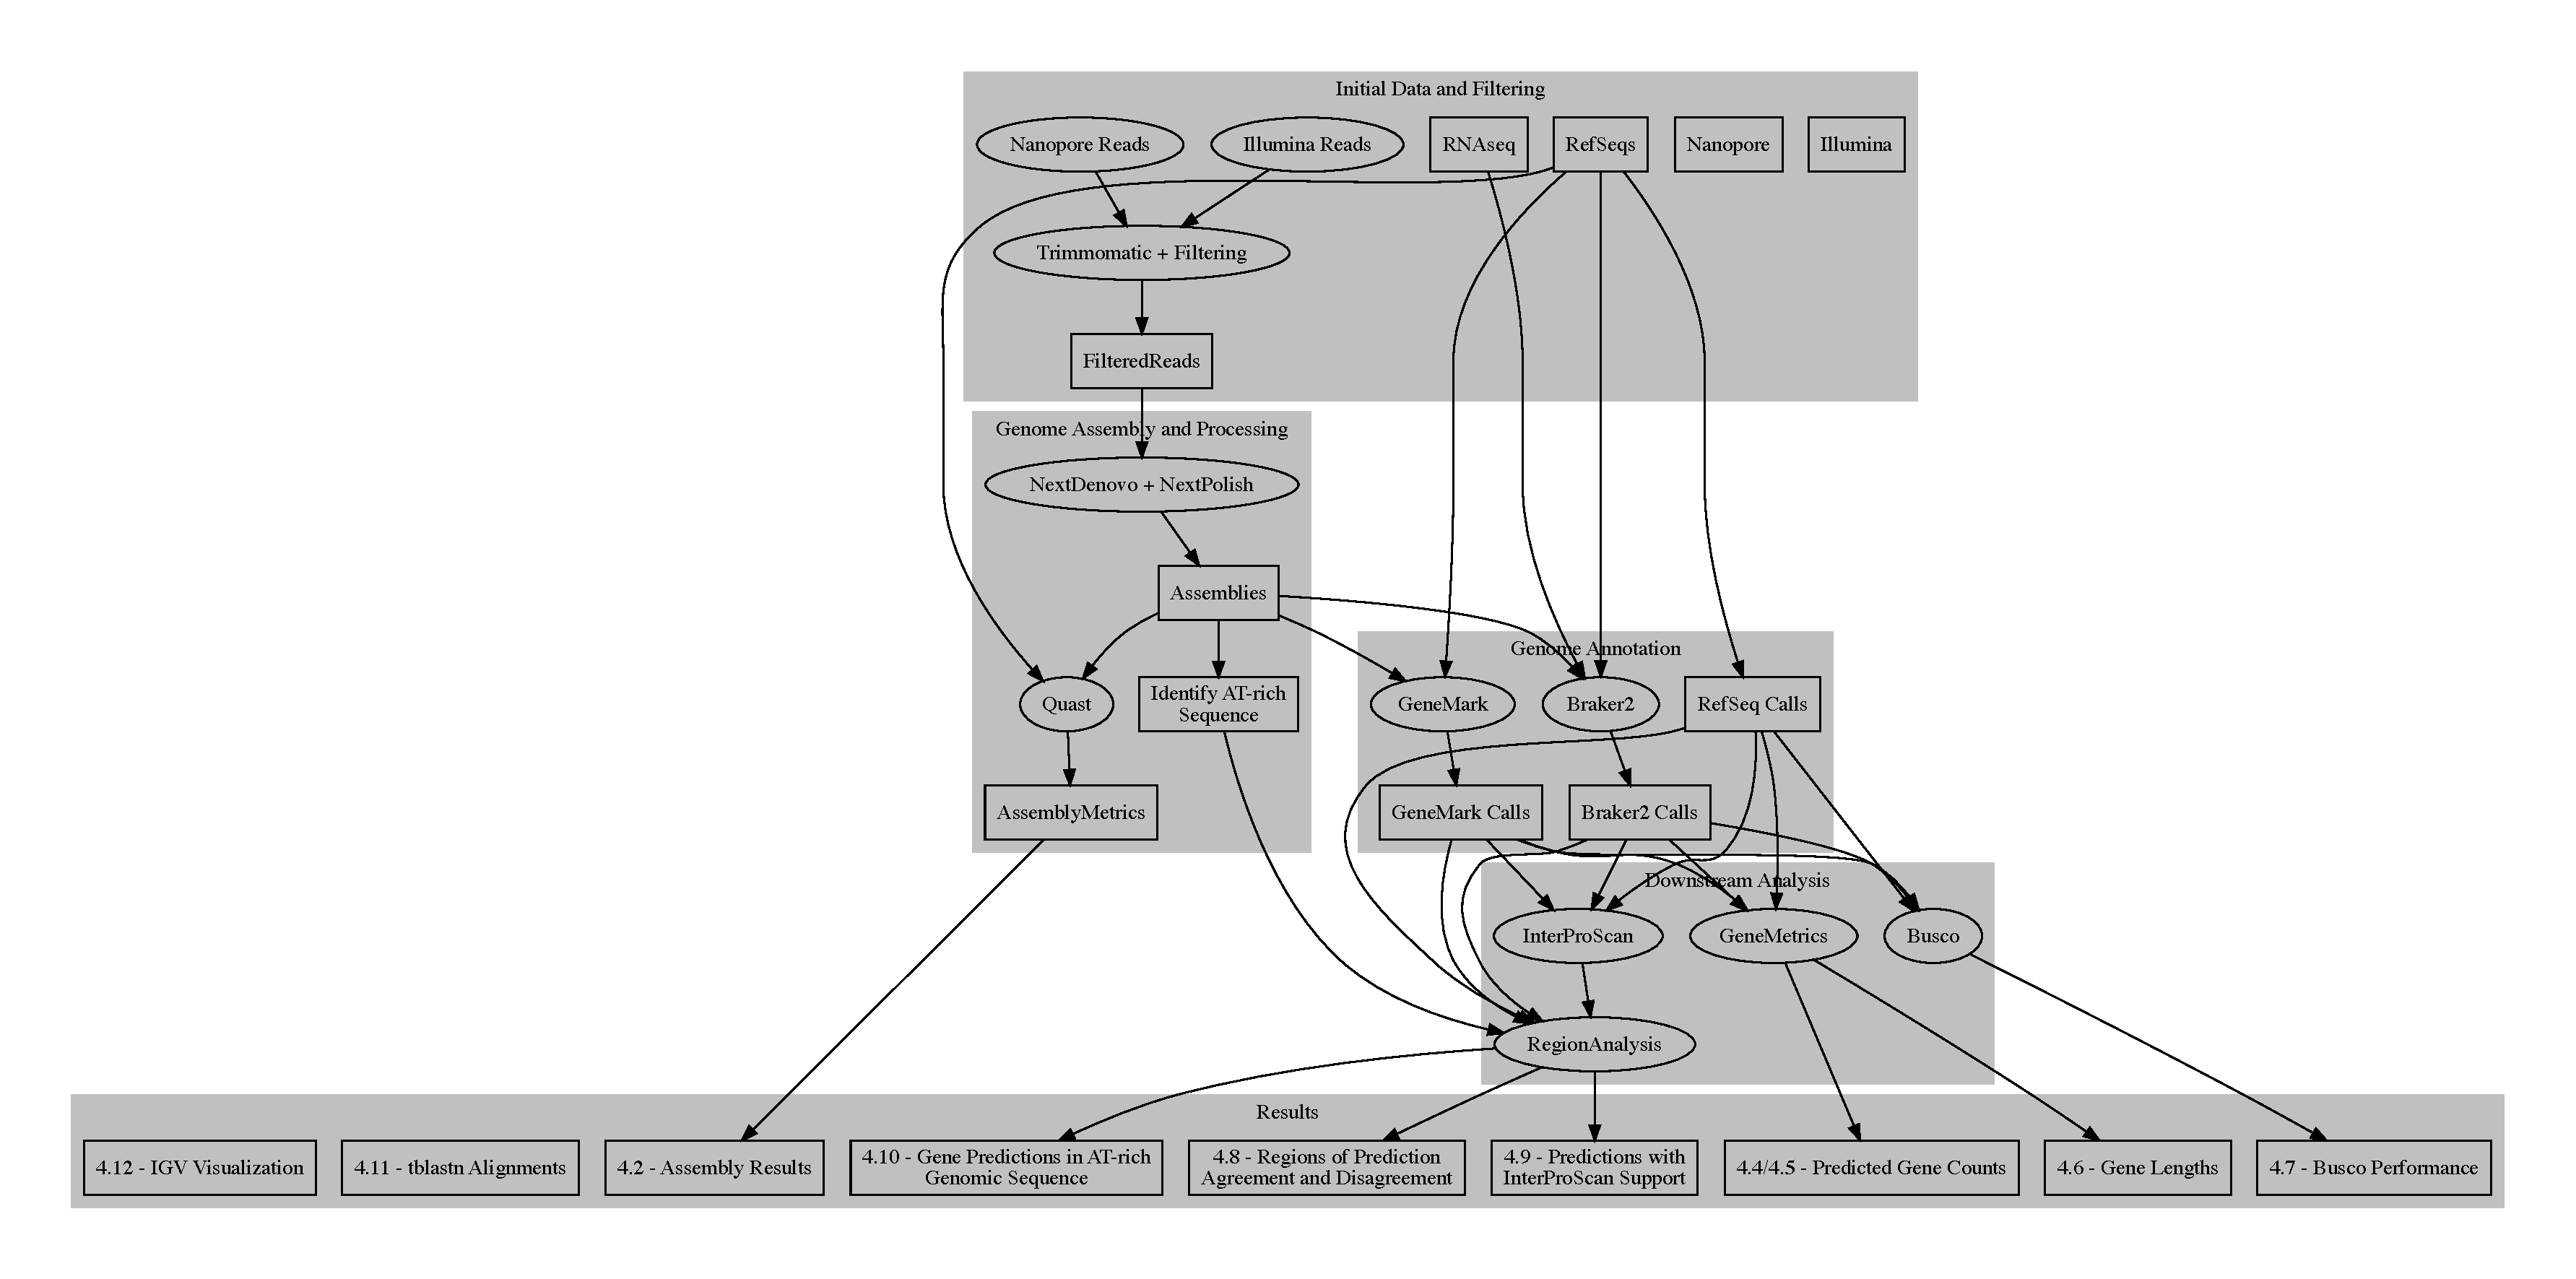
\includegraphics[width=1.25\textwidth]{./figures/data-flowchart.pdf}
%  }
%  \caption{A flowchart of the methodology followed in this
%    research. The workflow is broken up into sections based on the
%    processes and data involved at each step. Oval-shaped nodes
%    represent steps involved in the processing of data, while
%    rectangular nodes represent input and intermediate datasets as
%    well as results.}
%  \label{fig:workflow}
%\end{figure}

\section{Sequence Processing and Assembly Workflow}
\label{met:seq-workflow}

The sequence processing and assembly workflow is shown in Figure
\ref{fig:seq-workflow}. Processing steps are represented by boxes,
results of interest generated by this work are represented by folders,
and datasets that were not produced by this work are represented by
cylinders. Other workflows that use datasets produced by this workflow
are depicted as arrows outside of the brown sub-graph.

Illumina\textsuperscript{\textcopyright}\texttrademark
~\cite{bennett2004a} sequences were first trimmed and filtered using
Trimmomatic~\cite{bolger2014a} to remove adapter content and low-quality
sequences, as low-quality sequences may affect the assembly process,
resulting in fragmented and erroneous assemblies. The processed
Illumina\textsuperscript{\textcopyright}\texttrademark sequences and
Nanopore\textsuperscript{\textcopyright}\texttrademark~\cite{wang2021a}
sequences were then supplied to the hybrid genome assembly tool
NextDenovo~\cite{hu2024a}. As Ilumina sequences are of extremely high
accuracy, especially after trimming, the processed
Illumina\textsuperscript{\textcopyright}\texttrademark data was then
re-used to polish the assemblies with
NextPolish~\cite{hu2020a}. Polishing is used because long-read sequences
used in the assembly process are less accurate, at approximately
90-95\%, than Illumina sequences at ~99.9\%, so the Illumina data can
be used to correct any assembled sequences that may contain base-call
errors. The resulting assemblies were then analyzed to identify
AT-rich genomic sequence, analyzed with QUAST for general assembly
metrics, and then used as input in the gene prediction workflow.

The processing steps Trimmomatic filtering, NextDenovo assembly,
NextPolish Polishing and QUAST assembly assessment are described in
Section~\ref{met:seq-process}. The AT-rich sequence identification
process is described later in Section~\ref{met:atrich}.

\begin{figure}
  \centering
  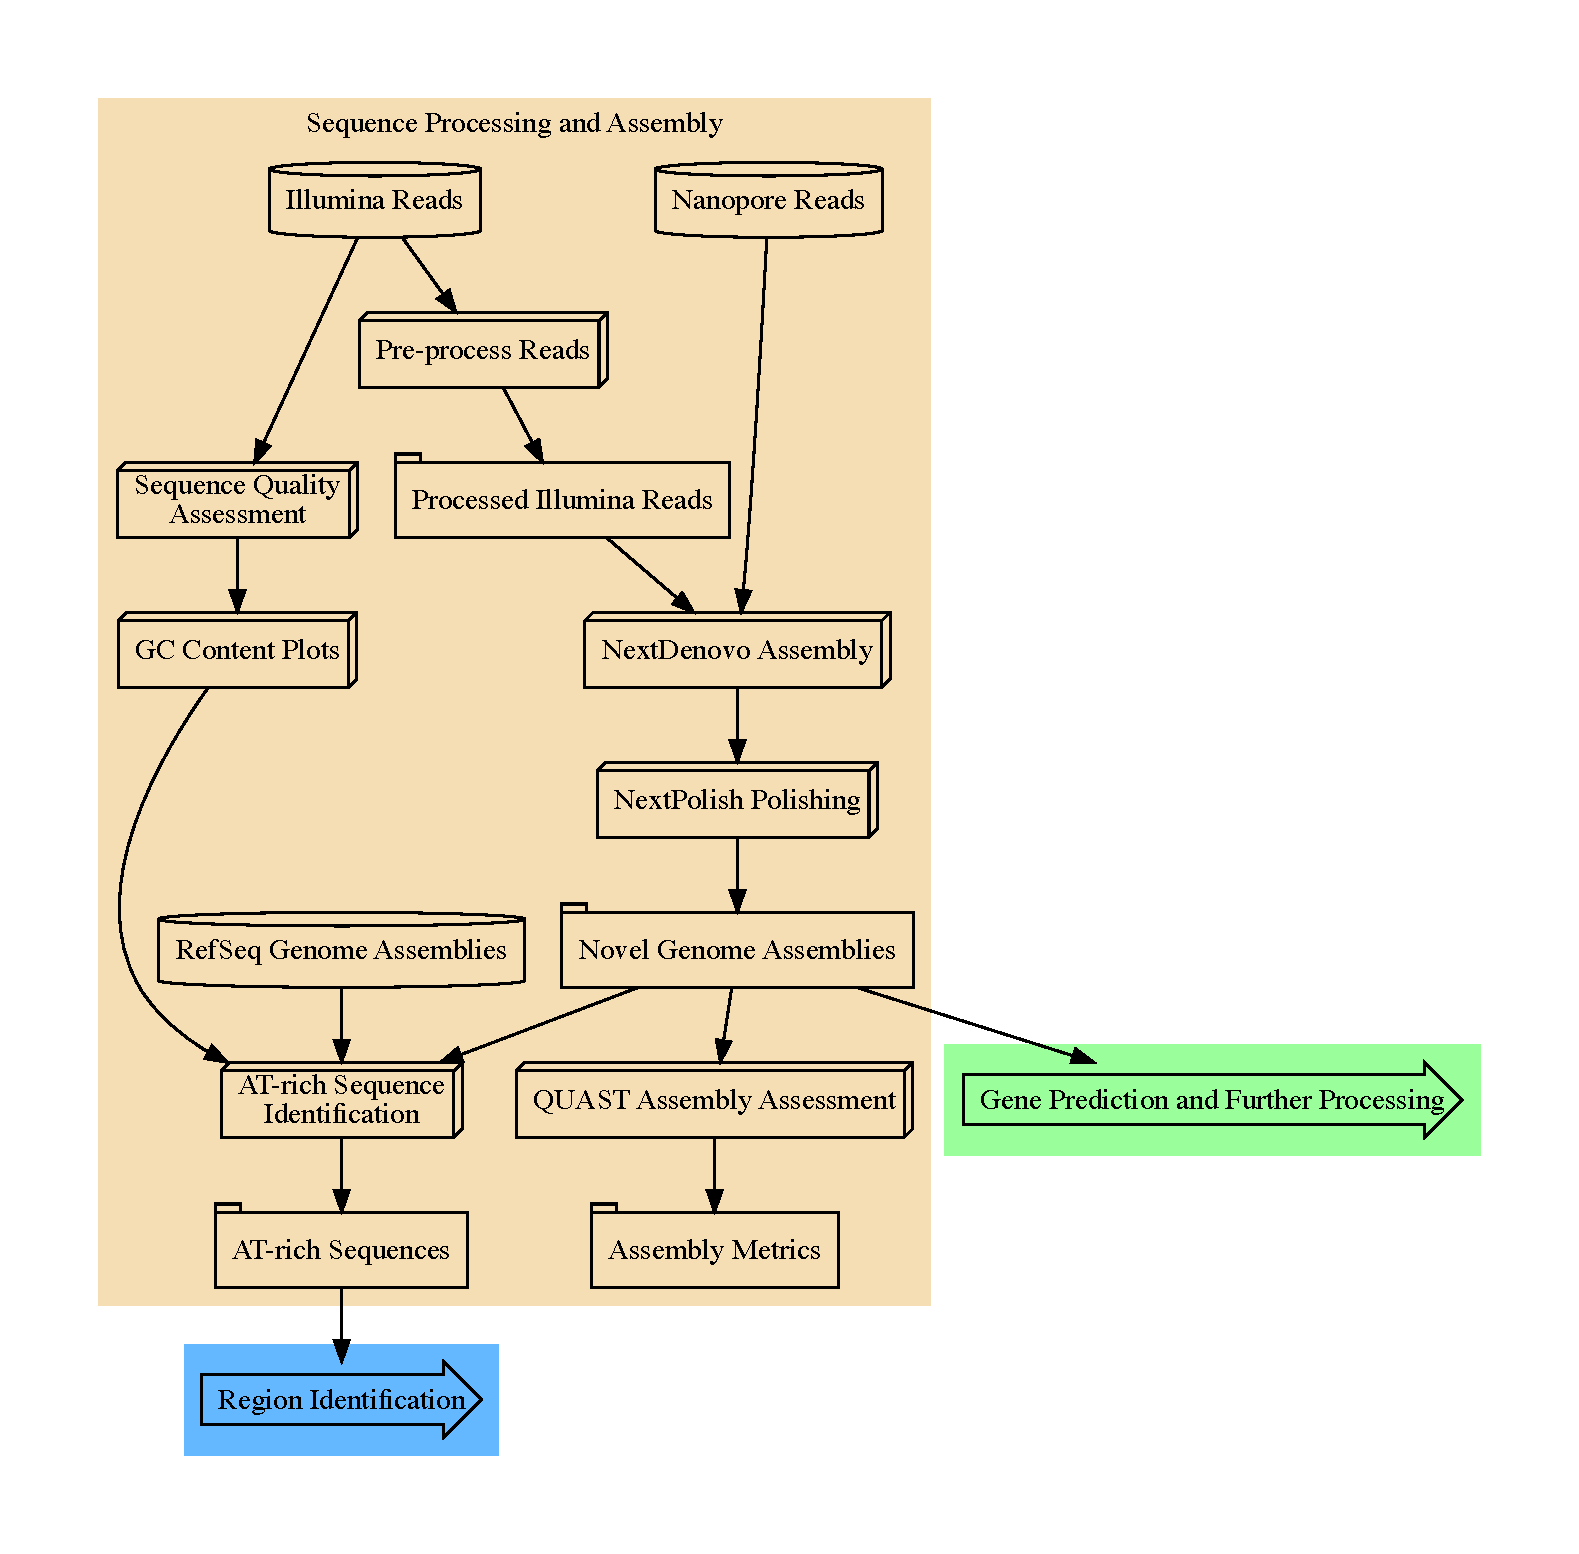
\includegraphics[width=\textwidth]{figures/assembly-met.pdf}
  \caption{A workflow (in brown) depicting the steps taken to process
    input sequences, generate assemblies, and post-process those
    assemblies for use in other workflows. Processing steps are
    represented by boxes, datasets of interest that were produced by
    this work are represented by folders, and datasets that were not
    produced in this work are represented by cylinders. Other
    workflows are represented by green and blue arrows outside of the
    brown graph. Directed edges indicate the flow of data.}
  \label{fig:seq-workflow}
\end{figure}

\subsection{Sequence Pre-processing and Assembly}
\label{met:seq-process}
% somewhere here...
% The training was performed using roughly 145 million Illumina
% paired end RNAseq reads on the \textit{Trichoderma reesei} genome.

Genomic sequences used for assembly were generated for DC1 and Tsth20
using
Nanopore\textsuperscript{\textcopyright}\texttrademark~\cite{wang2021a}
and
Illumina\textsuperscript{\textcopyright}\texttrademark~\cite{bennett2004a}
sequencing technologies by Brendan Ashby at the Global Institute for
Food Security at the University of Saskatchewan. Short-read sequences
were first examined with the FastQC tool~\cite{andrews} to evaluate
sequencing quality and general metrics associated with the sequencing
run. FastQC was run with default parameters. The short-read sequences
were then trimmed to remove any adapter content or low quality
sequences as they may lead to fragmented assemblies and erroneous base
calls.  Illumina\textsuperscript{\textcopyright}\texttrademark
sequencing data was filtered using Trimmomatic v0.38~\cite{bolger2014a}
with filtering criteria as follows: SLIDINGWINDOW:4:28, LEADING:28,
TRAILING:28, MINLEN:75. Only surviving paired-end reads were used for
further analysis. The
Nanopore\textsuperscript{\textcopyright}\texttrademark data were not
processed prior to assembly.

It has been shown that assemblies that use both short-read and
long-read sequencing data during the assembly are of higher quality
and less fragmented than assemblies using only one form of
sequencing. Genomic
Nanopore\textsuperscript{\textcopyright}\texttrademark and
Illumina\textsuperscript{\textcopyright}\texttrademark sequences from
DC1 and Tsth20 were assembled in to contigs using the hybrid assembly
tool
NextDenovo\textsuperscript{\textcopyright}\texttrademark~\cite{hu2024a}
v2.5.0 with default parameters. Although hybrid genome assemblies are
of higher quality, they may still contain base calling errors after
assembly. The highly accurate short-reads can be used to correct base
calling errors after assembly. To do this, the hybrid assemblies were
polished with Illumina\textsuperscript{\textcopyright}\texttrademark
sequences using NextPolish~\cite{hu2020a} v1.4.1 and default
parameters. Final assembly metrics were calculated using QUAST
v5.0.2~\cite{gurevich2013a} with default parameters.

\subsection{Identifying AT-rich Genomic Sequence}
\label{met:atrich}
Initial exploration of the Illumina sequence data generated for DC1
and Tsth20 showed bi-modal distributions of GC content in the
sequences. An example of the GC distribution of Illumina sequences for
DC1 is shown in Figure~\ref{fig:dc1-low-gc} compared to a theoretical
normal distribution. To differentiate AT-rich sequences from normal
sequences, a cutoff value was selected to isolate AT-rich sequences
from the rest. The cutoff value was chosen as 28\% GC content, which
is roughly the point where the AT-rich sequence counts begin
increasing in all assemblies. The details of this process are
explained below.

\begin{figure}
  \centering
  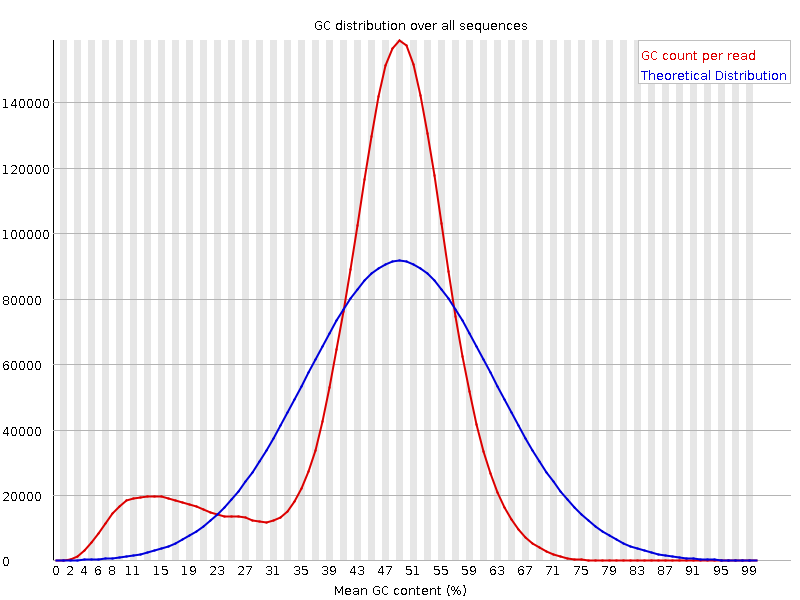
\includegraphics[width=\textwidth]{figures/dc1-low-gc-fastqc.png}
  \caption{A plot of GC content of Illumina sequences generated for
    DC1. The X-axis indicates mean GC content of sequences while the
    Y-axis indicates the total number of sequences for a given mean GC
    content. A theoretical normal distribution is overlaid in blue.}
  \label{fig:dc1-low-gc}
\end{figure}

AT-rich genomic sequences were identified using sliding windows of GC
content over each \textit{Trichoderma} assembly. Sliding windows were
generated using the isochore program from the EMBOSS tool suite
v6.6.0~\cite{rice2000a}. The sliding window used was 250bp wide with a
50bp shift. A window was classified as AT-rich if the sequence
contained lower than 28\% GC content. The genomic sequences from
AT-rich windows were mapped to a GFF file and processed using the
region identification algorithm described in section
~\ref{section:region-met}.

%In an attempt to produce high quality assemblies of DC1 and Tsth20, We
%decided on a set of tools named NextDenovo and NextPolish as they have
%produced excellent assemblies based on previous experience. (should
%find a citation to confirm this)

%(Might be better for discussion or omitted since it is specific to our
%setup) Initial attempts to run the example dataset resulted in
%permissions errors due to the management of the storage system being
%used, which were encountered with other tools in the past. To remedy
%this, the software installation was copied to RSMI's scratch space on
%Copernicus. Once the approriate permissions were given to run
%nextDenovo, the example dataset was run without issue.

%Following assembly using nextDenovo, Illumina sequence data from DC1
%and Tsth20 was used to polish each respective genome using
%nextPolish. Default parameters were used from assembly except for
%modification of the parallel option to reduce processing times.

%\subsection{Repeat Masking}

%In order to evaluate the performance of gene finding tools in
%repetitive or low complexity regions in the context of
%\textit{Trichoderma} genomes, we must first identify said regions in
%the genomes considered. To do this, the GenericRepeatFinder tool was
%used, which is a \textit{de novo} repeat detection tool
%\cite{10.1104/pp.19.00386}. GenerifRepeatFinder detects three
%different types of repeats, those being MITEs, TDRs and TIRs. Commands
%used for this program follow the example commands provided on the
%GitHub page for the GenericRepeatFinder project.


\section{Overview of Gene Prediction and Further Processing}
\label{met:predict-workflow}

To better understand the methods used in gene prediction and further processing, the steps have been assembled into a pipeline shown in Figure~\ref{fig:predict-workflow}. Processing steps are represented by boxes,
results of interest generated by this work are represented by folders,
and datasets that were not produced in this work are represented by
cylinders. Other workflows that use datasets produced by this workflow
are depicted as arrows outside of the green sub-graph.

First, RefSeq assemblies and their associated annotations of closely
related \textit{Trichoderma} species were selected from the National Center for Biotechnology Information (NCBI) for
training and comparison. Both \textit{ab initio}
(GeneMark~\cite{borodovsky2011a}) and evidence-based
(Braker2~\cite{bruna2021a}) gene finders were selected for comparison to
evaluate gene prediction behaviour of both methods in the context of
\textit{Trichoderma} genomes. Gene prediction was performed using both
gene finders on the RefSeq genomes and the genomes of DC1 and
Tsth20. Coding sequences output by the gene finders were then
examined to better understand distributions of CDS lengths produced by
different gene finders. Finally, all gene predictions were then
supplied to the evaluation and validation stage as well as the region
identification stage.

Datasets from the National Center for Biotechnology Information (NCBI) were selected for training and comparison, and are further
discussed in Subsection \ref{met:datasets}. The GeneMark gene prediction
process is described in Subsection \ref{met:genemark}, while the Braker2
gene prediction process is described in Subsection \ref{met:braker2}. The
process used to examine CDSs is described in Subsection \ref{met:cds-stats}.

\begin{figure}
  \centering
  \makebox[0pt]{
    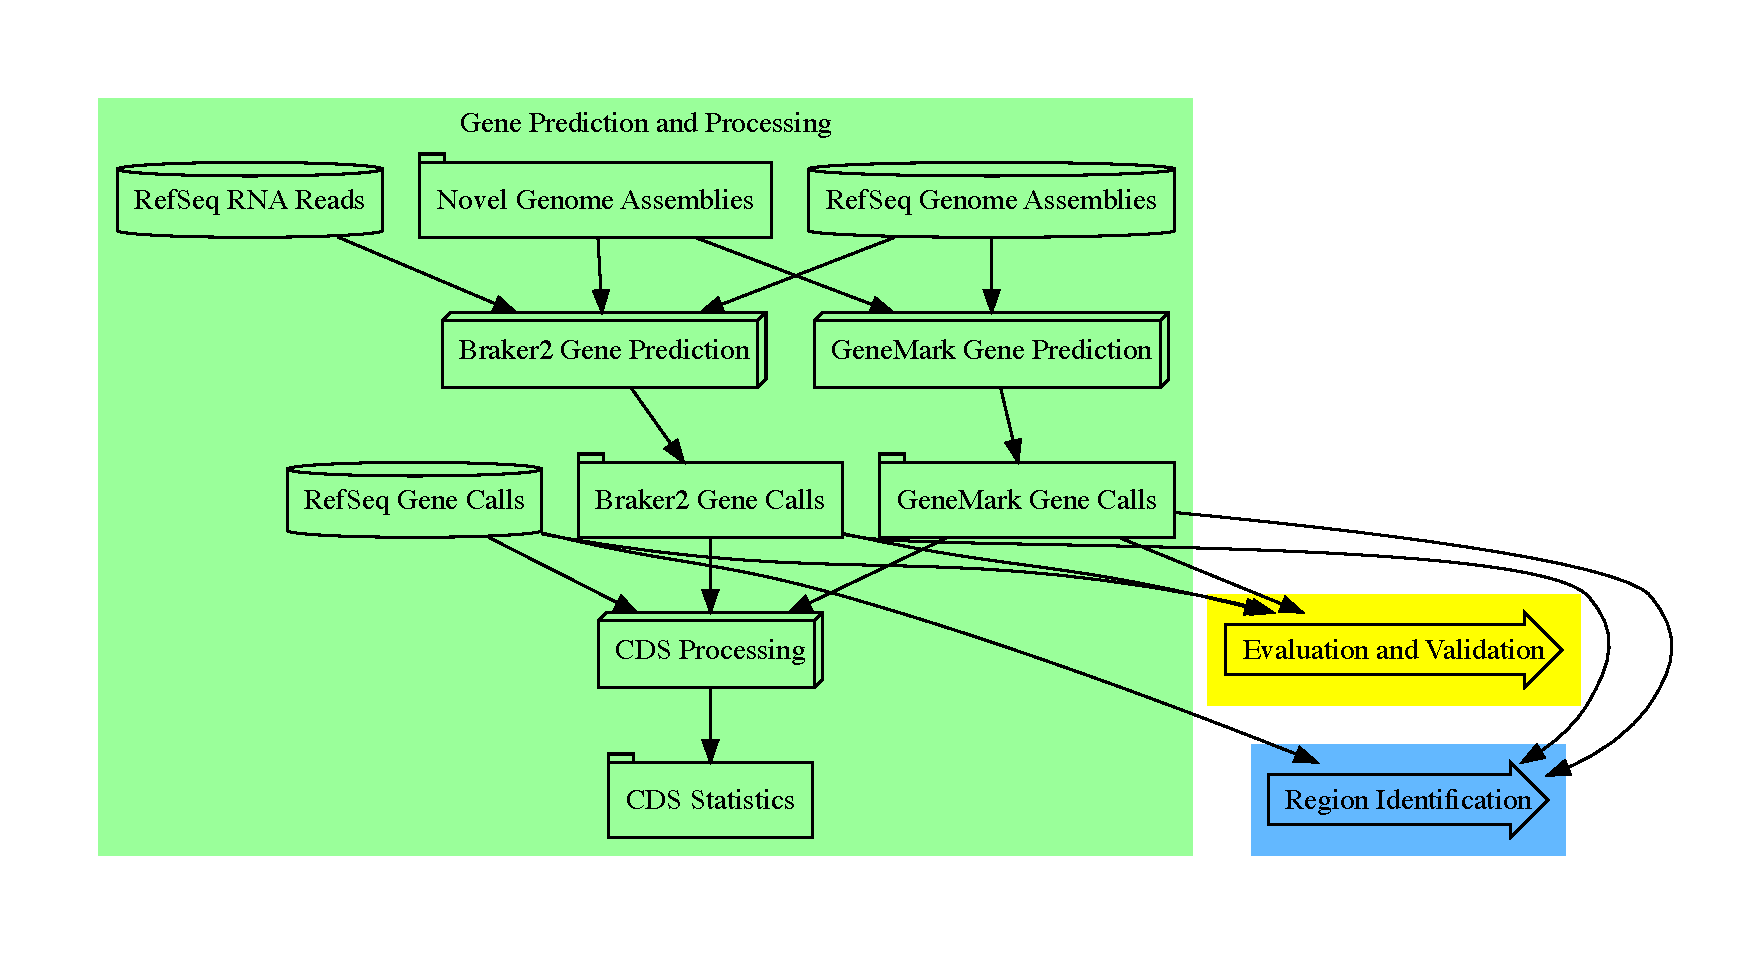
\includegraphics[width=\textwidth]{figures/gene-finding-met.pdf}
  }
  \caption{A workflow (green) depicting the steps taken to predict
    genes for use in other workflows and process CDS sequence
    lengths. Processing steps are represented by boxes, datasets of
    interest that were produced by this work are represented by
    folders, and datasets that were not produced in this work are
    represented by cylinders. Other workflows are represented by blue
    and yellow arrows outside of the green graph. Directed edges
    indicate the flow of data.}
  \label{fig:predict-workflow}
\end{figure}

\subsection{Selection of Datasets from NCBI}
\label{met:datasets}

When evaluating gene-finders, it is important compare gene predictions
to a standard, or control dataset, as a method of
ground-truthing. Such datasets include reference genome sequences and
their associated gene predictions from the NCBI as used in this work. In
addition to comparing against control datasets, RNAseq data can also
be used as training data for various tools as well, such as the
evidence-based training used by Braker2. In this work, four forms of
these inputs were selected from NCBI for comparison and training. The
first two datasets selected were assemblies and associated gene
predictions of three RefSeq \textit{Trichoderma} organisms, with
those organisms being \textit{T. virens}, \textit{T. harzianum}, and
\textit{T. virens}. NCBI RefSeq accession IDs for those assemblies are
GCF\_000167675.1\_v2.0, GCF\_003025095.1\_Triha\_v1.0, and
GCF\_000170995.1\_TRIVI\_v2.0, respectively. \textit{T. reesei} was
selected as it is the most well-studied \textit{Trichoderma} species,
and widely considered to be the gold-standard for \textit{Trichoderma}
genomes~\cite{gupta2016}. \textit{T. harzianum} and \textit{T. virens} were selected as additional datasets due to their prevalence in literature as well. It is important to note that while RefSeq is considered a high-quality
dataset, we did not use it as a ground truth in this case, but rather an additional point of comparison as it it possible that RefSeq annotations may also contain errors or omissions. This aligns with the method of region identification used later in this work, which is aimed to be a generic and adaptable method of comparing gene predictions, or any feature in GFF3 format, from multiple sources.

The second set of selected inputs were RNAseq datasets from 
\textit{T. reesei}, used as input in the training process for
Braker2. The use of training data in gene finding applications is to
produce a predictive model that factors in experimental evidence for a
`tailored' gene prediction model. These models can predict genes with
more confidence and predict the correct gene structure more
often~\cite{liang2009}. The SRA accession IDs for sequences used are:
SRR5229930, SRR8329344, SRR8329345, SRR8329346, and
SRR8329347. Limited RNAseq datasets were used as there were few RNAseq
datasets available at the beginning of this project.

The final set of inputs were protein sequences from RefSeq for the species
\textit{T. atroviride}, \textit{Fusarium graminarium}, and
\textit{Saccharomyces cerevisiae}, which were for downstream
validation of gene predictions.  The NCBI accession IDs for these
assemblies and associated protein sequences are GCF\_000171015.1,
GCF\_000240135.3, and GCF\_000146045.2, respectively.

\subsection{Gene Prediction Using GeneMark-ES}
\label{met:genemark}


\textit{Ab initio} gene finding was performed using GeneMark-ES
v4.71~\cite{borodovsky2011a} with DC1, Tsth20 and selected RefSeq
\textit{Trichoderma} assemblies used as input. Default parameters were
used in all cases except for the inclusion of the fungal option, which allowed the use
of a GeneMark model specific to fungal genomes.

%General command structure for GeneMark-ES:
%
%gmes\_petap.pl --ES --fungus
%--format gff3 --cores 48 --sequence /path/to/sequence

\subsection{Gene Prediction Using Braker2}
\label{met:braker2}

For evidence-based gene finding, Braker2 v3.0.2~\cite{bruna2021a} was
used with \textit{Trichoderma reesei} selected as the reference
organism for
training. Illumina\textsuperscript{\textcopyright}\texttrademark~\cite{bennett2004a}
RNAseq datasets from \textit{T. reesei} were downloaded from the NCBI
short-read archive using the sra-toolkit~\cite{zotero-item-326} and were not
trimmed or filtered prior to their use in Braker2 training. Default
parameters were used to train a Braker2 model on \textit{Trichoderma
  reesei} data except in the addition of the fungal option, which was used
for this analysis for improved gene-finding performance in fungi. The
trained Braker2 \textit{T. reesei} prediction model was then applied
to all assemblies with default parameters.

Braker2 also provides a UTR option to predict upstream sequence
features, but that option is experimental and was left off for this
work.

%The variables that need to be set are AUGUSTUS\_CONFIG\_PATH and
%TSEBRA\_PATH. Augustus, by defuault, tries to write species
%information to the location where the software is installed. In this
%case, we don'thave write permissions to the compute canada software
%stack hosted byt Research Computing, so the AUGUSTUS\_CONFIG\_PATH
%variable must be set in order to create a writeable directory. As long
%as that path has a directory within it called braker, and a species
%directory within the braker directory, things should go
%smoothly. TSEBRA is a set of scripts also made by the creators of
%Braker and is required to merge results from the various gene
%prediction tools involved in the Braker2 pipeline. The TSEBRA\_PATH
%simply points to the directory where TSEBRA is located Both Braker2
%and TSEBRA can be cloned directly from GitHub (links to come)

\subsection{Statistical Analysis of CDS Lengths}
\label{met:cds-stats}
The distribution of gene lengths predicted by a gene-finder is an
important feature to consider when selecting a gene finding tool, as
genes of a particular length may be of interest to researchers, but
more importantly, gene-finders may be biased to certain distributions
based on their underlying models. This is important as the
distribution of predicted gene lengths may also play a role in
\textit{Trichoderma's} role as an avirulent plant symbiont. These
biased distributions may differ from the true distribution of CDS
lengths leading to propagation of sub-optimal gene-finding results and
results that may not reflect the true distribution of gene lengths. To
determine, if differences exist between distributions of predicted
gene lengths from each tool, the $\log_{10}$ lengths of coding
sequences (CDS) were subject to a two-sample Kolmogorov-Smirnov
test~\cite{2008}. The null hypothesis of this test is that the number of genes in AT-rich and normal GC content regions should be proportional to the length of AT-rich and normal GC content regions in the genome.

\section{Overview of Evaluation and Validation of Gene Predictions}
\label{met:valid-workflow}

Following the gene prediction process, prediction results can then be
evaluated and used as queries against exiting datasets as a form of
validation. 

Coding sequences from the previous stage were evaluated and validated
using several tools. Firstly, protein products from predicted CDSs
were processed with InterProScan to identify Pfam domains as evidence
for the validity of gene predictions. Secondly, CDSs were analyzed
with BUSCO to assess prediction of conserved fungal genes. Finally,
RefSeq proteins from related fungal species were used in tblastn
searches of the five \textit{Trichoderma} assemblies selected for the
main body of this work.

BUSCO evaluation, InterProScan Annotation, and BLAST alignments
processes are described in more detail in Subsections ~\ref{met:busco},
~\ref{met:interproscan}, and ~\ref{met:blast}, respectively. Results
from these processes are also used as inputs in the region
identification workflow later.

\begin{figure}
  \centering
  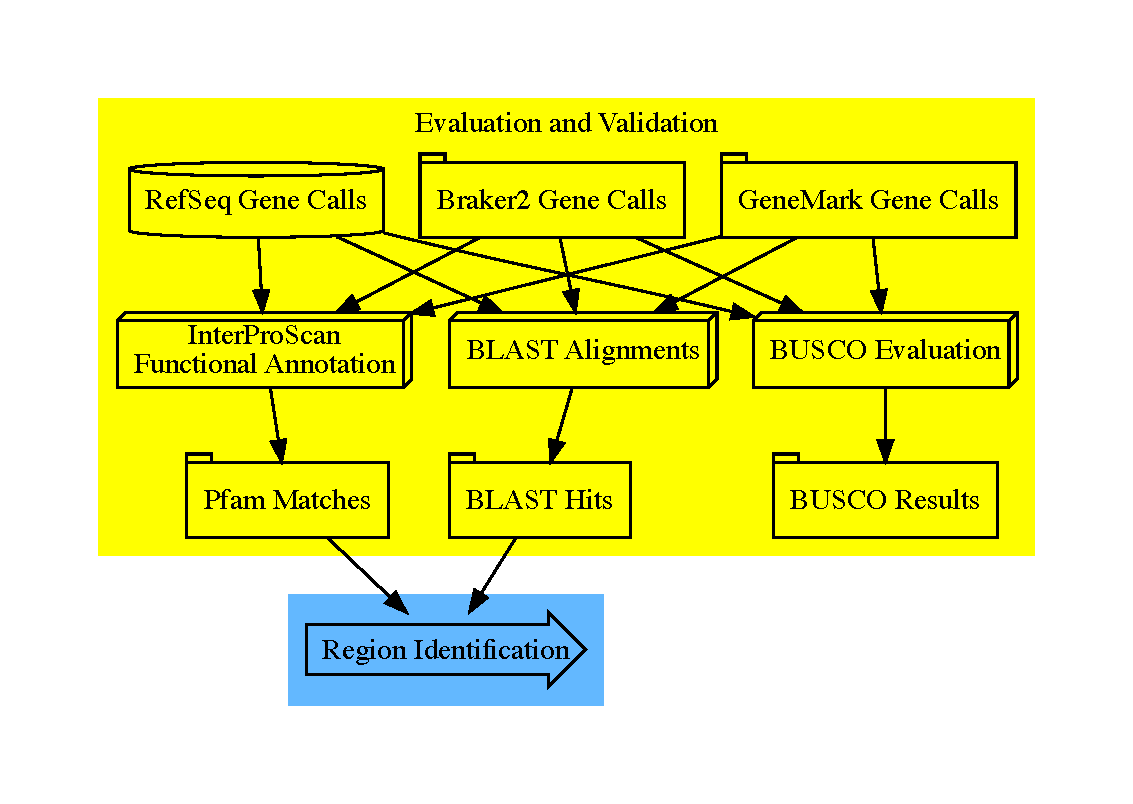
\includegraphics[width=0.8\textwidth]{figures/eval-met.pdf}
  \caption{A workflow (yellow) depicting the steps taken to evaluate
    and validate predicted genes. Processing steps are represented by
    boxes, datasets of interest that were produced by this work are
    represented by folders, and datasets that were not produced in
    this work are represented by cylinders. Other workflows using
    results from these processing steps are represented by a
    blue arrow outside of the yellow graph. Directed edges
    indicate the flow of data.}
  \label{fig:valid}
\end{figure}

\subsection{Evaluating Gene-Finder Performance Using BUSCO}
\label{met:busco}
While novel gene predictions are of great interest in new subjects, it
is also important to confirm that gene-finders are predicting genes
that are expected to be present in the organism of
interest~\cite{manni2021b}. To determine if this
is true, BUSCO v6.0.0~\cite{simao2015a} was selected
as a tool to determine a gene-finder's ability to predict a set of
conserved orthologous genes. The BUSCO Metaeuk pipeline was run using default parameters with the BUSCO sordariomycetes\_Odb12 fungal lineage dataset to capture highly
conserved genes in fungal genomes closely related to \textit{Trichoderma} species. This pipeline was applied to all
genome assemblies used in this work.

\subsection{Functional Annotation Using InterProScan}
\label{met:interproscan}
The presence of a functional component in a predicted gene's protein
product is good evidence in favour of a gene-finder's performance. To
identify functional components, the protein products from each gene
finder's predictions were functionally annotated using InterProScan
v5.65-97.0~\cite{jones2014} without the match
lookup service and with the following analyses included: AntiFam-7.0,
CDD-3.20, Coils-2.2.1, FunFam-4.3.0, Gene3D-4.3.0, Hamap-2023\_01,
MobiDBLite-2.0, NCBIfam-13.0, PANTHER-18.0, Pfam-36.0, PIRSF-3.10,
PIRSR-2023\_05, PRINTS-42.0, ProSitePatterns-2022\_05,
ProSiteProfiles-2022\_05, SFLD-4, SMART-9.0,
SUPERFAMILY-1.75. InterProScan was run on all predicted proteins using
default parameters. The resulting protein annotations were mapped back
to their genome assemblies and processed using the region
identification algorithm in section ~\ref{section:region-met}.

\subsection{Ground-truthing with the Basic Local Alignment Search Tool (BLAST)}
\label{met:blast}
The \textit{Trichoderma} assemblies chosen for comparison were used as
the subject sequences in tblastn~\cite{gertz2006} searches with the query proteins discussed in paragraph three of Section ~\ref{met:datasets}. Default parameters were used in the tblastn searches. Hits from the tblastn alignments were then filtered for alignments with a minimum of 30\% query coverage and 30\% identity. These criteria were selected as they filter out spurious alignments while also retaining short alignments that capture functional or conserved protein coding sequence. Remaining alignments were then processed using the region identification algorithm in ~\ref{section:region-met}. In the third row, are the AT-rich sequences identified in Section ~\ref{met:atrich}, the tblastn alignments identified in Subsection ~\ref{met:blast}, and the Pfam matches from InterProScan identified in Subsection ~\ref{met:interproscan}.

\section{Region Identification Overview}
\label{section:region-overview}
A major portion of this work was the process of identifying regions of
overlapping features as a method of comparing gene calls from
different gene prediction tools. The definition of a region and the algorithm
used to identify them is described in detail in Section
~\ref{section:region-met}, and an overview of the region identification
workflow is shown in Figure~\ref{fig:region-overview}. The top of the
graph shows the gene calls produced by the workflow described in
Subsection~\ref{met:predict-workflow}, which are used as the main input
to the region identification process. The inputs and resulting regions of other previously
generated datasets is represented within the rounded rectangles. These additional datasets may contain other
information such as BLAST alignments or functional annotations and can
be included as features in the region identification process. Regions output by the region identification process
were then visualized with the Integrative Genomics Viewer, described
in Section~\ref{section:igv-met}

\begin{figure}
  \centering
  \makebox[0pt]{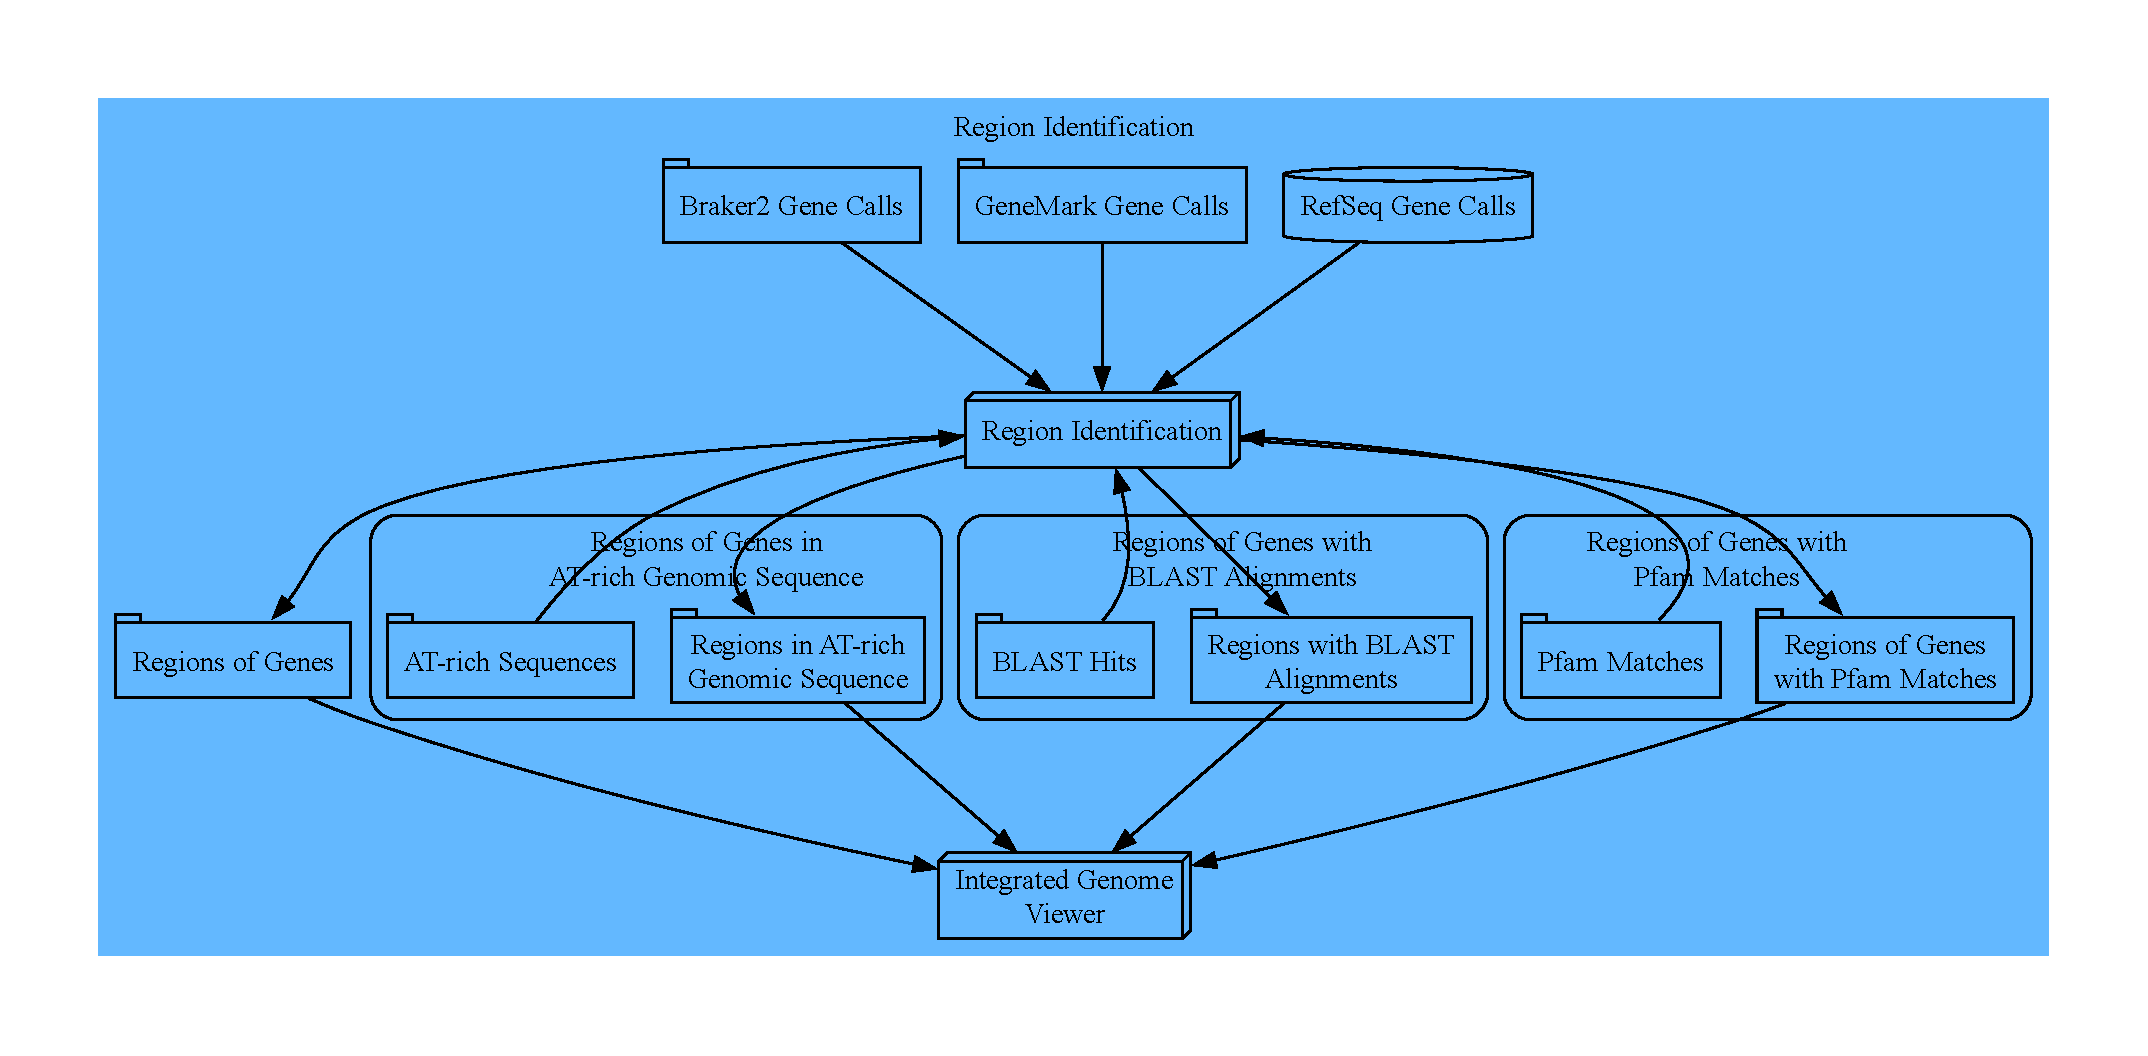
\includegraphics[width=1.2\textwidth]{figures/region-workflow.pdf}}
  \caption{An overview of the region identification process for
    different datasets. Sections of the graph are outlined with
    rounded rectangles, indicating that the datasets within were processed
    along with gene calls and discussed in their own results
    sections. Processing steps are represented by boxes, datasets of
    interest that were produced by this work are represented by
    folders, and datasets that were not produced by this work are
    represented by cylinders. Directed edges indicate the flow of
    data.}
  \label{fig:region-overview}
\end{figure}


\subsection{Region Identification Algorithm}
\label{section:region-met}

The gene predictions Subsections ~\ref{met:datasets}~\ref{met:braker2}, ~\ref{met:genemark}, and the additional datasets from Subsections ~\ref{met:atrich}, ~\ref{met:blast}, ~\ref{met:interproscan} were processed into regions of overlapping gene predictions. A region is defined as a pair of genomic coordinates containing one 5$'$ and one 3$'$ coordinate, between which are one or more overlapping features.
We define a feature as a pair genomic
coordinates containing one start and one stop coordinate that is
associated with a gene prediction, annotation, or other information of
interest.

Overlapping features were processed into regions using a concept
similar to Allen's interval algebra~\cite{dechter2003}. The
algorithm first sorts all features on each contig by start coordinate
and then iterates over each feature, identifying overlaps with
previous features to identify regions of overlapping features. We
approached this as a graph problem, where features make up a set of
nodes \textit{V}, and spatial overlaps between features make up a set
of edges \textit{E}, forming the graph \textit{G} = \textit{\{V,
    E\}}. This algorithm performs a transitive closure
\textit{R}\textsuperscript{+} of \textit{G}, resulting in sub-graphs,
or regions of features in which each node has a path to each other
node in that sub-graph. Pseudo-code for the algorithm is shown in
Algorithm~\ref{alg:regions}. This processing was performed with Python
v3.12.4~\cite{foundationa} and the GFF package from BCBio~\cite{chapmana}
for easy GFF parsing. The resulting regions were then further
processed to identify trends and behaviours of gene finders in the
context of other annotated information and features.

\begin{algorithm}
  \begin{algorithmic}
    \State INPUT:\ list\ of\ GFF\ files,\ $GFFList$
    \State RETURNS:\ list\ of\ regions,\ $regionList$
    \For{\texttt{<each GFF in GFFList>}}
    \State $allFeatures \gets GFF.features$
    \EndFor
    \State $sortedFeatures \gets sortStartCoord(allFeatures)$
    \State $regionList \gets []$
    \State $firstFeature \gets firstItem(sortedFeatures)$
    \State $lastFeature \gets lastItem(sortedFeatures)$
    \For{\texttt{<each feature in sortedFeatures>}}
      \If{$feature = firstFeature$}
        \State $currentRegion \gets newRegion(feature)$
        \State $currentRegion.start \gets feature.start$
        \State $currentRegion.end \gets feature.end$
      \ElsIf{$feature = lastFeature$}
        \State $regionList.append(currentRegion)$
        \State $return\ regionList$
      \ElsIf{$feature\ overlaps\ currentRegion$}
        \State $currentRegion.updatePositions(currentRegion, feature)$
        \State $currentRegion.addFeature(feature)$
      \Else
        \State $regionList.append(currentRegion)$
        \State $currentRegion \gets newRegion(feature)$
        \State $currentRegion \gets feature.start$
        \State $currentRegion \gets feature.end$
      \EndIf
    \EndFor
    \State $return\ regionList$
  \end{algorithmic}
  \caption{The general algorithm underlying the region identification
    process.}
  \label{alg:regions}
\end{algorithm}

\subsection{Regions in AT-rich Genomic Sequence}
\label{met:atrich2}
AT-rich genomic sequence regions were identified using the
process described in Subsection~\ref{met:atrich} and were used input to the region identification process.

\subsection{Visualization of Identified Regions}
\label{section:igv-met}
Results from the region identification process were visualized using
the IGV genome browser v2.19.1~\cite{robinson2011a}. An example of an
IGV screenshot is shown in Figure~\ref{fig:igv-methods}.

\begin{figure}
  \centering
  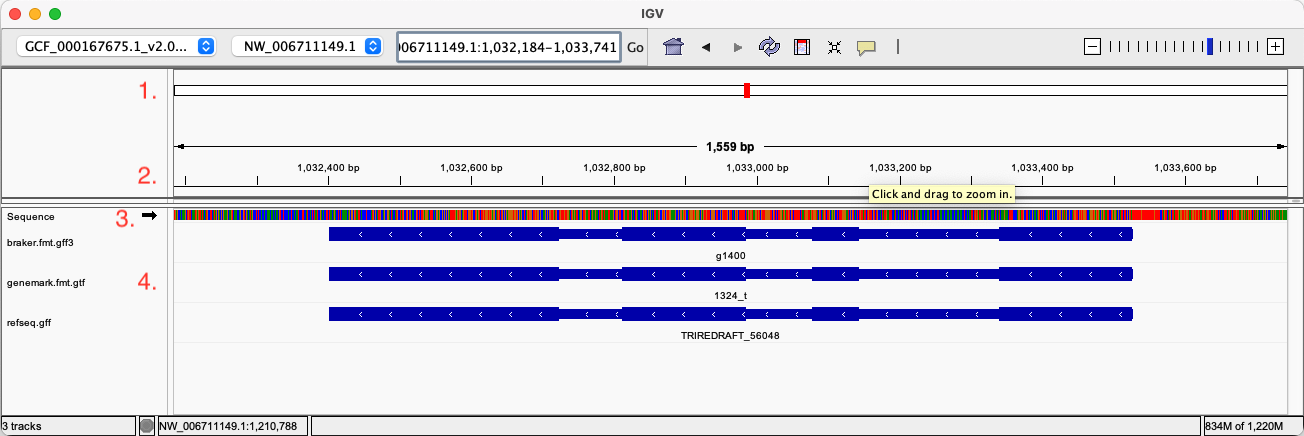
\includegraphics[width=0.9\textwidth]{figures/igv/igv-agreement-thin-number}
  \caption[IGV example]{An example of an IGV screenshot used in
    portions of the results from this work. The top half of the image
    displays information about the reference sequence with track one
    showing the position of the viewer relative to the reference
    sequence, and track two showing the numerical positions of the
    reference. The lower half of the image displays more tracks in the
    form of additional layers of information mapped to the reference
    sequence. Track three shows a track displaying the nucleotide at
    each position if the scale of the viewer is small enough. Track
    four comprises several tracks, each containing features, the
    regions in blue, from a GFF file. The tracks in this example are
    limited to gene predictions, although tracks in other IGV
    screenshots may include features from other tools such as
    InterProScan and will be discussed in their respective
    sections. Individual tracks will be referred to in increasing
    numerical order in the track list beginning from the top. The
    nucleotide track is not included in the order.}
  \label{fig:igv-methods}
\end{figure}

%=======
%Example command for braker2:
%
%/scratch/p2irc/p2irc\_rsmi/cbe453/masters/software/braker2/BRAKER/scripts/braker.pl
%--gff3 --threads 60
%--TSEBRA\_PATH=/scratch/p2irc/p2irc\_rsmi/cbe453/masters/software/braker2/tsebra/TSEBRA/bin/
%--genome /path/to/sequence --species=TreeseiFungal --fungus
%--useexisting
%
%BUSCO methodology (from research questions)
%The BUSCO method was applied using two BUSCO subsets,
%one generally applicable for fungi, and another targeting an
%evolutionary branch more closely related to \textit{Trichoderma}.
%
%Stats for length analysis (from research questions)
%The first statistical tool to be applied is ANOVA (analysis of
%variance) to compare the mean lengths genes predicted by each gene
%finding tool with the null hypothesis being that the mean of predicted
%gene lengths should be the same across all tools considered. In
%addition to ANOVA, pairwise comparisons of the distributions using a
%Kolmogorov–Smirnov test is appropriate. The null hypothesis in this
%test would be that the gene lengths are sample from the same
%distribution.
%
%Stats for binomial tests (from research questions)
%To do this, a binomial test will be used, with the null hypothesis
%being that the number of genes predicted in regions of normal and
%abnormal GC content should be proportional to the length of normal and
%abnormal GC content regions in the assembly. For example, if 30
%percent of the genome is comprised of anomalous GC content, then we
%would expect 30 percent of predicted genes to be present in those
%regions. In addition to anomalous GC content, this test can be applied
%to repetitive content in assemblies as well.
%
%Stats for regions (from research questions)
%From these results, Venn diagrams will be generated with
%Jaccard index calculated for each combination of gene finding
%tools. The region identification process can also be extended to
%include features identified by other tools, such as BLAST hits to
%validated gene models from other organisms and small RNAs. Chi2
%goodness of fit tests can then be applied to counts of 'validated'
%gene predictions or other features with the same null hypothesis that
%gene finders should predict the same number of features.
